\section{Example}
A study concerns the approval ratings of a prime minister in two
surveys.
In the first survey, ratings were obtained on 1600 citizens and
then in a second survey, six months later, the same citizens were
resurveyed.

\begin{itemize}
	\item In the 1st survey, 944 indicated approval of the Prime Minister's
	performance in office.
	\item In the 2nd survey, 880 indicated approval.
\end{itemize}

There each subject has two observation. So that we have 1600 pairs of data out of 1600 people.

\begin{figure}[H]
	\centering
	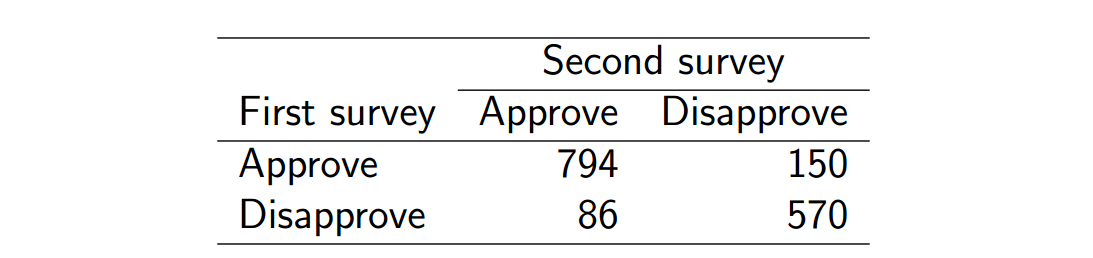
\includegraphics[width=0.7\linewidth]{fig/screenshot010}
	\caption{Contingency Table}
	\label{fig:screenshot010}
\end{figure}

The null hypothesis is 
\[H_0: \text{the approval rate does not change.}\]
It can be reduced to
\[H_0: \text{the odds of approval does not change.}\]
It means that the probability of going from approval to disapproval is the
same as the probability of going from disapproval to approval.

In the following code, we identify that 4 more percentage of people going from approval to disapproval. McNemar test tells us that it is significant.

\lstinputlisting[language=R]{code/l12-exp4.R}

kappa test focus on the agreement while the McNemar Test focus on the disagreement.

\lstinputlisting[language=R]{code/l12-exp5.R}